% !TeX root = skript.tex
Ein Zufallsgraph ist ein Modell einer Graphfamilie --- etwa wie eine Zufallsvariable ein Modell einer Zufallsgröße ist.
Der Zufallsgraph beschreibt also ein Ensemble von Graphen, das so entworfen sein kann, dass bestimmte Eigenschaften in den betrachteten Graphen verstärkt auftreten.
So maßgeschneiderte Zufallsgraphen werden oft als \emph{Netzwerkmodell} bezeichnet.

Das Forschungsfeld der Zufallsgraphen nahm mit den Arbeiten von Gilbert~\cite{gilbert_1959}, sowie Erd\H{o}s und R\'enyi~\cite{erdos_renyi_1960} Anfang der 1960er Jahre an Fahrt auf.
Die beiden Arbeiten definieren Zufallsgraphen, die zunächst für abstrakte Untersuchungen (z.B. die Probabilistische Methode) verwendet wurden.
Der Fokus auf die Modellierung von beobachteten Netzwerken kam erst später hinzu.
Dennoch spielen die Modelle in der Netzwerkforschung bis heute eine wichtige Rolle.
Wir werden sie daher bald genauer betrachten, fangen jedoch mit einem noch einfacheren Modell an.

\section{Der Zufallsgraph $\Gn$}
Ein Zufallsgraph $(\mathbb G, P)$ ist eine Wahrscheinlichkeitsverteilung $P\colon \mathbb G \to [0, 1]$ über einer Menge von Graphen $\mathbb G$.
Oftmals wird der Grundraum $\mathbb G$ durch eine Parametrisierung eingeschränkt; auch $P$ kann parametrisiert sein.

Das \aside{$\Gn$ Graphen} einfachste Modell ist $\Gn$, welches die Gleichverteilung über alle Graphen mit $n$ Knoten beschreibt.
Hierbei ist zu beachten, dass wir mit \emph{alle Graphen} in der Regel entweder alle \emph{gerichteten} oder alle \emph{ungerichteten} Graphen meinen.
Die Details der Analysen in den folgenden Kapiteln hängen von dieser Entscheidung ab --- allerdings ergeben sich meist keine qualitativen Unterschiede.
Daher werden wir oft den für uns einfacheren Fall wählen.
Je nach Wahl, ist der Grundraum von $\Gn$
\begin{eqnarray}
    \mathbb G_\text{ger}(n) &=&
    \twoset{G(V,E)}{|V| = n \land E \subseteq V \times V}\\
    \mathbb G_\text{unge}(n) &=&
    \twoset{G(V,E)}{|V| = n \land  E \subseteq \twoset{\set{u,v}}{u,v \in V \text{ mit } u \ne v}}.
\end{eqnarray}

\noindent Die Wahrscheinlichkeitsverteilung $P$ folgt dann als $P_{\gGn}(G) = 1 / | \gGn |$, oder konkret:
\begin{eqnarray}
    P_{\mathbb G_\text{ger}(n)}(G) &=& \frac{1}{| \mathbb G_\text{ger}(n) |} = \frac{1}{n^2}\\
    P_{\mathbb G_\text{unge}(n)}(G) &=& \frac{1}{| \mathbb G_\text{unge}(n) |} = \frac{1}{\binom n 2} = \frac{2}{n(n-1)}.
\end{eqnarray}

\begin{figure}[t]
    \begin{center}
        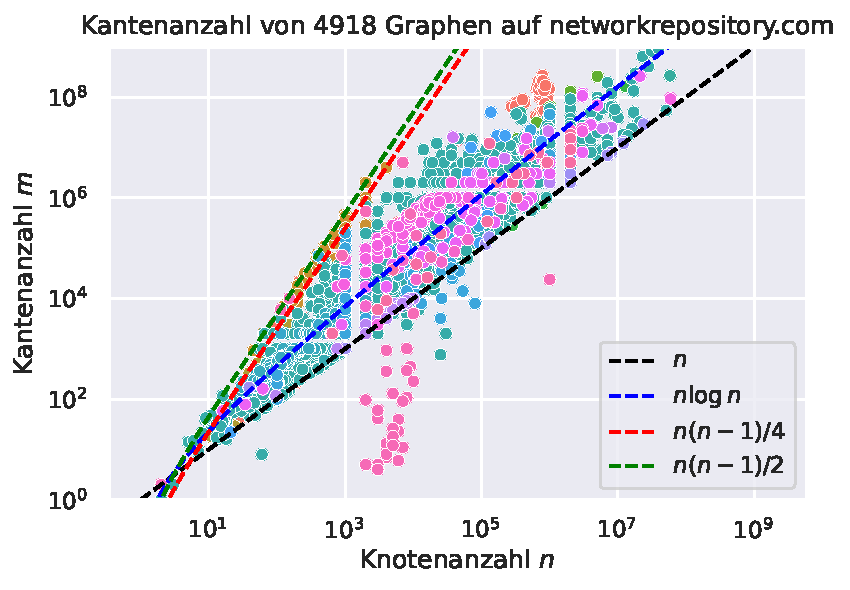
\includegraphics[width=0.5\textwidth]{data/network-rep-edges.pdf}%
        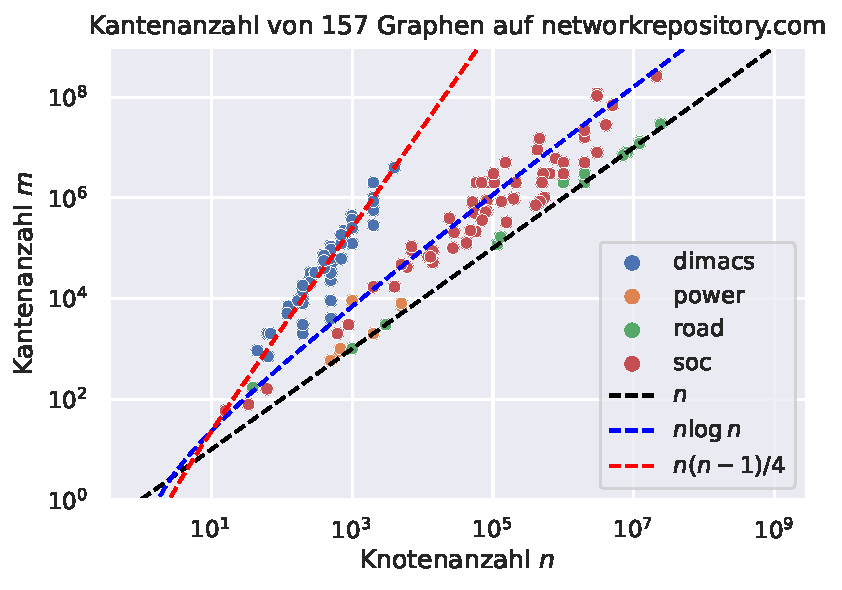
\includegraphics[width=0.5\textwidth]{data/network-rep-edges-thin.pdf}%
    \end{center}
    \caption{
        Die Verteilung der Kantenanzahl in verschiedenen Netzwerken auf~\cite{networkrepository}.
        Die Farben der einzelnen Punkte geben an, aus welchem Bereich die Netzwerke stammen.
    }
    \label{fig:kantenanzahl}
\end{figure}

Ist das $\Gn$ Modell realistisch?
Das hängt davon ab, was wir mit ihm bezwecken und was wir mit \emph{realistisch} meinen.
Es ist aber sicherlich nicht geeignet, um gängige Netzwerke zu beschreiben.
Dies liegt unter anderem daran, dass $\Gn$ oft Graphen mit vielen Kanten erzeugt;
intuitiv hat \glqq jeder zweite Graph\grqq{} mindestens die Hälfte aller möglichen Kanten.

\begin{observation}
    Sei $G(V,E)$ ein Graph, der zufällig aus $\Gn$ mit $n > 1$ gezogen wurde.
    Dann gilt für gerichtete Graphen $\prob{|E| \ge n^2 / 2} \ge 1/2$ und für ungerichtete Graphen $\prob{|E| \ge \binom{n}{2} / 2} \ge 1/2$.
\end{observation}

\begin{proof}
    Im Folgenden betrachten wir nur gerichtete Graphen; der Beweis läuft analog für ungerichtete Graphen.
    Stellen wir uns einen beliebigen Graphen~$G(V, E)$ vor.
    Dann sei $\bar G(V, \bar E)$ sein Komplement, d.h. für alle möglichen Kanten gilt:
    \begin{equation}
        \forall e \in V\times V\colon \quad\quad e \in \bar E \Leftrightarrow e \notin E
    \end{equation}
    Beobachte, dass es eine Bijektion zwischen allen Graphen in $\mathbb G$ und ihren Komplementen gibt: jeder Graph hat ein eineindeutiges Komplement.
    Per Konstruktion gilt außerdem:
    \begin{eqnarray}
        E \cup \bar E &=& V \times V\\
        \Rightarrow |E| + |\bar E| &\ge& n^2\\
        \Rightarrow \max(|E|, |\bar E|) &\ge& n^2 / 2.
    \end{eqnarray}

    Für jeden Graph~$G$ gilt also, dass entweder $G$ selbst oder sein Komplement~$\bar G$ mindestens $n^2 / 2$ Kanten hat.
    Da wir $G$ und $\bar G$ je mit gleicher Wahrscheinlichkeit ziehen, gilt $\prob{|E| \ge n^2 / 2} \ge 1/2$.
\end{proof}

\section{Kantenanzahl in beobachteten Netzwerken}\label{sec:kanten-in-beobachteten-netzen}
Wie viele Kanten haben echte Netzwerke? Hierzu führen wir ein Experiment durch:
wir nutzen die Datenbank \url{https://networkrepository.com/}, die über 5000 Netzwerke aus unterschiedlichen Bereichen enthält~\cite{networkrepository}.
In \cref{fig:kantenanzahl} zeichnen wir die Kantenanzahl als Funktion der Knotenanzahl.
Zwei Eigenschaften fallen direkt auf:
\begin{enumerate}
    \item Die Kantendichte hängt vom Netzwerktyp ab.
    \item Es sind fast immer deutlich weniger als die Hälfte der Kanten vorhanden.
\end{enumerate}

\subsection{Netzwerktypen haben unterschiedliche Kantendichten}
Betrachten wir die erste Beobachtung genauer, indem wir Straßennetze und Freundschaftsnetze vergleichen.
Wir modellieren ein Straßennetz dadurch, dass Adressen (Häuser, Kreuzung, usw.) als Knoten und Straßen als Kanten dargestellt werden.
Diese Netze \aside{Straßennetze} sind im wesentlichen ein zwei-dimensionales Konstrukt.
Wenn wir Tunnel, Brücken und der gleichen ignorieren, verlaufen Straßen nicht über einander.
Daher erwarten wir, dass die Graphen von Straßennetzen fast planar sind.
Nach dem Eulerischen Polyedersatz erfüllen einfache, \aside{planare Graphen} planare und zusammenhängende Graphen:
\begin{equation}
    |E| \le 3 |V| - 6
\end{equation}
Knoten in einem Straßennetz sollten also im Schnitt höchstens 6 Nachbarn haben.

In \aside{Freundschaftsnetze} sozialen Netzwerken ist die Situation anders ---
stellen wir uns etwa einen Freundschaftsgraphen vor, in dem Knoten die Nutzer eines sozialen Netzwerks sind und Kanten eine Freundschaft anzeigen.
Im Jahr 2014, hatten Facebook-Nutzer im Schnitt mehr als 300 Freunde (mehr dazu später).
Dies ist offensichtlich deutlich mehr als in planaren Graphen möglich wäre.
Ganz ähnlich sieht es mit anderen sozialen Netzen aus: ein durchschnittlicher Erwachsener kennt deutlich mehr als 6 andere Menschen persönlich (oft werden Zahlen zwischen 100 und 300 genannt).

\subsection{Die meisten Netzwerke sind dünn}
In \cref{fig:kantenanzahl} hat nur ein verschwindend geringer Anteil der Netzwerke mindestens die Hälfte aller Kanten (d.h. ist oberhalb der roten Linie).
Wie erklärt sich das?
In der Regel verursacht eine Kante Kosten:
eine Straße muss gebaut werden, eine Freundschaft muss aufrecht erhalten werden (Zeitinvestment), eine Nachricht muss geschrieben werden, etc.
Daher gibt es in den meisten Netzwerken einen gewissen Selektionsdruck, der dazu führt, dass jeder Knoten nur ausgewählte Nachbarn besitzt.

\begin{definition}
    Graphen \aside{dünne und dichte Graphen} mit $n$ Knoten und $m$ Kanten heißen \emph{dünn} (engl. sparse), wenn $m = \Oh{n \log n}$ gilt, und \emph{dicht} wenn $m = \Omega(n^2)$.
\end{definition}

\begin{remark}
    Aufgrund der asymptotischen Definition verwendet man \emph{dünn} und \emph{dicht} eher für Graphfamilien (so auch Zufallsgraphen) als für einzelne Instanzen.
    Manche abweichende Definitionen fordern für \emph{dünne} Graphen $m = \Oh{n}$.
    Wir nutzen hier $\Oh{n\log n}$, um soziale Netzwerke mit einzubeziehen.
\end{remark}

\section{Die Zufallsgraphen $\Gnm$ und $\Gnp$}
Das $\Gn$ Modell verfügt über keinen Mechanismus um Kanten auszudünnen.
Wir benötigen also Prozesse, die weniger dichte Graphen erzeugen können ---
am besten parametrisiert, damit wir unterschiedlichen Netzwerktypen Rechnung tragen können.
Im Folgenden betrachten wir zwei solcher Modelle.

Das \Gnm-Modell \aside{Erd\H{o}s-R\'enyi Graphen \Gnm} von P.~Erd\H{o}s und A.~R\'enyi beschreibt die Gleichverteilung über alle Graphen mit $n$ Knoten und $m$ Kanten, d.h. wir betrachten die Grundmenge
\begin{equation}
    \gGnm = \twoset{G(V,E)}{G(V,E) \in \Gn \text{ und } |E| = m}.
\end{equation}
Da gleichverteilt gewählt wird, gilt für die Verteilungsfunktion~{$P\colon \mathbb G \to [0,1]$} einfach
\begin{equation}
    P(G) = \frac{1}{| \gGnm |} \quad \text{ für alle } G \in \gGnm.
\end{equation}

\begin{exercise}
    Berechne $|\gGnm|$ für gerichtete und ungerichtete Graphen.
\end{exercise}

E.~Gilbert \aside{Gilbert-Graphen \Gnp} beschrieb ein ähnliches Modell, das \Gnp-Modell --- das oft fälschlicherweise \glqq Erd\H{o}s-R\'enyi-Modell \grqq{} genannt wird.
Um das Modell zu beschreiben, weichen wir von der bisherigen expliziten Definition der Grundmenge und Verteilung ab.
Stattdessen, spezifizieren wir eine randomisierte Konstruktionsvorschrift:
\begin{enumerate}
    \item Erzeuge $n$ Knoten $V = \{v_1, \ldots, v_n\}$.
    \item Setze $E = \emptyset$.
    \item Für jedes Paar von Knoten $(v_i, v_j)$ führe ein Bernoulli Experiment durch.
          Mit Wahrscheinlichkeit $p$ füge $(v_i, v_j)$ unabhängig als Kante zu $E$ hinzu.
    \item Gebe den Graphen $G=(V, E)$ zurück.
\end{enumerate}

\noindent
Graphisch kann man sich also \Gnp als Adjazenzmatrix vorstellen, in der die Einträge unabhängig voneinander mit Wahrscheinlichkeit $p$ auf $1$ gesetzt werden:

\begin{center}
    \begin{tikzpicture}
        \node (mat) at (0,0) {
            $\begin{pmatrix}
                    1 & 0 & 1 & 0 & 0 \\
                    0 & 1 & 1 & 0 & 1 \\
                    0 & 1 & 0 & 1 & 0 \\
                    1 & 0 & 1 & 0 & 0 \\
                    1 & 0 & 0 & 0 & 1 \\
                \end{pmatrix}$
        };

        \node[anchor=west, align=left, xshift=4em] (label) at (mat.east) {
            $\begin{cases}1 & \text{mit Wahrscheinlichkeit } $p$ \\
                    0 & \text{mit Wahrscheinlichkeit } 1-p
                \end{cases}$
        };

        \path[draw, thick, bend right, ->] (label.west) to (mat.center);
    \end{tikzpicture}

\end{center}

\begin{exercise}
    Die genannte Konstruktion erzeugt gerichtete Graphen.
    Zeige, wie die Konstruktion so angepasst werden kann, dass gerichtete Graphen ohne Eigenschleifen erzeugt werden.
    Wie verändert sich dann die Adjazenzmatrix?
    Wie verhält es sich mit ungerichteten Graphen?
\end{exercise}

Durch ihre einfache Konstruktion sind beide Zufallsgraphen bis heute sehr verbreitete Modelle in der Netzwerkforschung.
Wir werden jedoch sehen, dass viele Eigenschaften von echten Netzwerken auch von \Gnp oder \Gnm-Graphen nicht beschrieben werden können.

\subsection{Anzahl von Kanten in \Gnp}
Während bei \Gnm Graphen die Anzahl der Kanten durch den Parameter~$m$ fixiert ist, ist $|E|$ bei \Gnp Graphen eine Zufallsvariable.

\begin{lemma}\label{lemma:erwartete_kanten_in_gnp}
    Die \aside{Erwartete Kantenanzahl $\expv{|E|}$ in \Gnp} erwartete Anzahl an Kanten in einem gerichteten \Gnp Graphen ist \begin{equation*} \expv{m} = p n^2. \qedhere \end{equation*}
\end{lemma}

\begin{proof}
    Fixiere einen Graphen~$G=(V,E)$ aus \Gnp.
    Für jede Kante $(u,v)$ definiere die Indikatorvariable $I_{u,v}$, die anzeigt, ob die Kante $(u,v) \in E$ enthalten ist:
    \begin{equation}
        I_{u,v} = \begin{cases}
            1 & \text{ falls } (u,v) \in E \\
            0 & \text{ sonst }
        \end{cases}
    \end{equation}

    \noindent Somit folgt Anzahl der Kanten~$m$ in $G$ als Summe über die Indikatorvariablen
    \begin{equation}
        m = \sum_{u,v \in V} I_{u,v} = \left(\sum_{(u,v) \not\in E} 0 \right) +  \left(\sum_{(u,v) \in E} 1\right) = |E|.
    \end{equation}

    \noindent Per Definition von \Gnp gilt $\prob{I_{u,v} {=} 1} = p$ und $\prob{I_{u,v} {=} 0} = 1-p$.
    Somit folgt für den Erwartungswert jeder Indikatorvariable
    \begin{equation}
        \expv{I_{u,v}} = 1 \cdot p + 0 \cdot (1-p) = p \quad \text{unabhängig für alle } u, v \in V.
    \end{equation}

    \noindent Durch die Linearität des Erwartungswertes folgt schließlich
    \begin{equation}
        \expv{|E|} = \sum_{u,v \in V} \expv{I_{u,v}} = \sum_{u,v \in V} p = p n^2. \qedhere
    \end{equation}
\end{proof}

\begin{exercise}
    Zeige, dass die erwartete Anzahl an Kanten in einem ungerichteten \Gnp Graphen $\expv{m} = \binom{n}{2} p = p n(n-1)/2$ beträgt.
\end{exercise}

\begin{exercise}
    Zeige, dass $\Gn = \mathcal G(n, 1/2)$.
\end{exercise}

\bigskip

Wie wir am Beweis von \cref{lemma:erwartete_kanten_in_gnp} sehen, ergibt sich die Kantenanzahl~$m$ als Summe von unabhängigen Bernoulli Zufallsvariablen;
sie ist also selbst eine Zufallsvariable und binomial verteilt.
Da uns die Binomialverteilung regelmäßig begegnen wird, wollen wir uns diese kurz in Erinnerung rufen.
\begin{definition}
    Die \aside{Binomialverteilung.} Binomialverteilung $B_{N, p}(k)$ beschreibt die Wahrscheinlichkeit, dass bei $N$~unabhängigen Bernoulli Experimenten mit Wahrscheinlichkeit $p$ genau $k$ Experimente erfolgreich sind.
    Es gilt \aside{\ \\ \ \\ \ \\ Binomialkoeffizient $\binom{n}{k} = \frac{n!}{(n-k)!k!}$}
    \begin{eqnarray*}
        \prob{B_{N,p} {=} k} &=& \binom{N}{k} p^k (1-p)^{N-k} \\
        \expv{B_{N,p}} &=& Np \\
        \varv{B_{N,p}} &=& Np(1-p),
    \end{eqnarray*}
    wobei $\expv{B_{N,p}}$ und $\varv{B_{N,p}}$ den Erwartungswert und die Varianz der Binomialverteilung beschreiben.
\end{definition}

Die Standardabweichung $\sigma = \sqrt{\varv{B_{N,p}}} \le \sqrt{\expv{B_{N,p}}}$ ist also relativ klein.
Wir können daher davon ausgehen, dass für hinreichend großes $N$ die Binomialverteilung recht stark um ihren Erwartungswert $Np$ konzentriert ist.
Daher sagen wir, dass \Gnm und \Gnp mit $p=m/n^2$ asymptotisch (d.h. für $n \to \infty$) äquivalent sind.
Häufig ist es jedoch einfacher \Gnp Graphen zu analysieren, da ---im Gegensatz zu \Gnm Graphen--- alle Kanten unabhängig gezogen werden.

\section{Effizientes Ziehen von \Gnp Graphen}
Zufallsgraphen sind nicht nur in der theoretischen Analysen von Prozessen und Algorithmen nützlich, sondern auch für empirische Untersuchungen.
Nehmen wir etwa an, dass wir einen Algorithmus implementiert haben und dessen Geschwindigkeit oder Qualität vermessen möchten.
Dann können Zufallsgraphen unter anderem aus folgenden Gründen nützlich sein:
\begin{itemize}
    \item Wenn die Generatorsoftware vorhanden ist, können wir synthetische Instanzen in quasi unbeschränkter Menge generieren.
    \item Parametrisierte Generatoren erlauben den Einfluss gewisser Eigenschaften detailliert zu analysieren; z.B. Skalierungsexperimente.
    \item Beobachtete Graphen haben oft \glqq Rauschen\grqq, d.h. nicht verstandene oder insignifikante Strukturen, die Messungen verfälschen können.
          Zufallsgraphen, hingegen, haben i.d.R. eine gut verstandene Struktur, die es uns oft ermöglicht vor dem Testen Hypothesen aufzustellen.
    \item Einige Generatoren können anhand eines fixierten Startzustands (Random-Seed) dieselben Graphen wiederholt erzeugen.
          Wir müssen also die Eingaben nicht speichern/transferieren und können dennoch reproduzierbare Experimente durchführen.
\end{itemize}

\noindent Da in verschiedenen wissenschaftlichen Communities der Begriff \glqq Generator\grqq{} unterschiedlich benutzt wird, hier noch eine Definition:
\begin{definition}
    Ein \aside{Graphgenerator} Graphgenerator ist ein Algorithmus, der einen Graphen aus einem Netzwerkmodell erzeugt.
    Dieser respektiert die Verteilung des zugrundeliegenden Modells.
\end{definition}

\subsection{Ein naiver Ansatz}
Betrachten wir folgenden Graphgenerator für \Gnp Graphen, der im wesentlichen eine 1:1 Implementierung der Definition von \Gnp ist:

\begin{algorithm}[H]
    \KwIn{Anzahl der Knoten~$n$ und Verbindungswahrscheinlichkeit~$p$}
    \KwOut{Adjazenzmatrix eines zufälligen Graphs $G \follows G(n, p)$}
    Allokiere eine Matrix $A[1..n, 1..n]$\;
    \For{$1 \le i \le n$}{
        \For{$1 \le j \le n$}{
            Setze $A[i,j] \gets \begin{cases}
                    0 & \text{mit Wahrscheinlichkeit } 1-p \\
                    1 & \text{mit Wahrscheinlichkeit } p
                \end{cases}$\;
        }
    }
    Gebe $A$ zurück
    \caption{Naiver Graphgenerator für \Gnp Graphen}
    \label{alg:naive-gnp}
\end{algorithm}

Um \aside{Annahme: aus einfachen Verteilungen kann in kostanter Zeit gezogen werden.} die Laufzeit dieses Algorithmus bestimmen zu können, treffen wir in dieser Veranstaltung folgende Annahme.
Wir können unter anderem aus folgenden Zufallsverteilungen in konstanter Zeit ziehen:
\begin{itemize}
    \item Ganzzahlig uniform aus $[a, b]$ für $a, b \in \mathbb{Z}$.
    \item Gleitkommazahl uniform aus $[a, b]$ für $a, b \in \mathbb{R}$.
    \item Bernoulli (folgt aus vorherigem Punkt)
    \item Binomial, Geometrisch (siehe \cref{{sec:inversionsmethode}}), Hypergeometrisch, Poisson
\end{itemize}

Tatsächlich können die meisten dieser Verteilungen nur in \emph{erwartet} konstanter Zeit gezogen werden, praktisch sind die Fluktuationen jedoch so klein, dass wir sie vernachlässigen können.
Das erlaubt es uns auf die Eigenschaften der Graphgeneratoren zu konzentrieren.

\begin{lemma}
    \label{lem:naive-gnp}
    Der Algorithmus \ref{alg:naive-gnp} erzeugt einen \Gnp Graphen in $\Theta(n^2)$ Zeit.
\end{lemma}

\begin{exercise}
    Beweise das Lemma.
\end{exercise}

Nun könnte man argumentieren, dass dieser naive Algorithmus bereits optimal ist:
Die Ausgabe hat Größe $\Theta(n^2)$ und somit wir benötigen $\Omega(n^2)$ Zeit, um die Ausgabe zu erzeugen.
Außerdem hat ein Graph mit $p=\Omega(1)$ erwartete $\Theta(n^2)$ Kanten, was wiederum die Laufzeit von unten beschränkt.

Diese Worst-Case Schranken passen jedoch nicht zu unserer Beobachtung in \cref{sec:kanten-in-beobachteten-netzen}, dass Graphen in der freien Wildbahn meist dünn sind.
Es wäre schön, wenn wir diese Graphen schneller erzeugen könnten, jedoch ist \cref{alg:naive-gnp} für alle $p$ gleich \glqq schnell\grqq.
Hier \aside{ausgabesensitive Algorthmen} helfen \emph{ausgabesensitive Algorithmen} (output-sensitive algorithm), deren Laufzeit maßgeblich durch die Größe der Ausgabe bestimmt wird;
die meisten Generatoren, die wir betrachten werden, fallen genau in diese Kategorie.

Ausgabesensitive \aside{Kantenlisten} Algorithmen müssen jedoch eine Ausgabedatenstruktur nutzen, die sich an die Größe anpasst.
Eine Matrix hat immer dieselbe Größe unabhängig davon, wie viele Einsen (Kanten) vorhanden sind.
Wir werden im Folgenden fast immer eine Kantenliste annehmen, die nur $\Oh{1}$ Speicherworte pro Kante benötigt.

\subsection{Ziehen mit zufälligen Sprüngen}
Wie können wir nun \cref{alg:naive-gnp} verändern, so dass er ---analog zu Kantenlisten--- keine Arbeit für Nichtkanten verrichtet?
Idee: Wir müssen diese einfach überspringen!
Aber woher wissen wir wo \glqq Nullen\grqq{} gezogen werden, bzw. wie viele Nullen müssen wir überspringen?
Zählen können wir sie nicht ohne wieder direkt quadratische Arbeit zu verrichten.

Ganz einfach: wir fragen uns wie viele Nullen~$\ell$ \cref{alg:naive-gnp} gesetzt hätte und überspringen diese.
Zwischen diese zufälligen Sprünge setzen wir dann die Einsen ein.
Wenn wir nun $\ell$ aus einer geeigneten Verteilung ziehen, haben wir zwei unterschiedliche Zufallsprozesse, deren Ausgabe aber nicht unterscheidbar ist.
Generalisierungen dieser Methode werden uns noch häufiger begegnen.

Zur Vereinfachung, stellen wir uns die Adjazenzmatrix~$A = (a_{ij})_{ij}$ als einen Vektor~$B = (b_k)_k$ vor, der dadurch entsteht, dass wir die Zeilen hinter einander anfügen.
Eintrag $a_{ij}$ wird also mit $b_{(i-1)n + j}$ identifiziert.
Dann besteht unsere Aufgabe darin genau alle $b_k$ zu finden, die den Wert $1$ haben.

\begin{equation}
    \Big(\quad \cdots \overbrace{1}^{b_k} \ \underbrace{0 \ \ 0\ \ 0 \ \cdots\ \ 0\ \ 0\ \ 0}_{\text{$\ell$ zusammenhängende Nullen}}\  \overbrace{1}^{b_{k + 1+ \ell}} \cdots \quad \Big)
\end{equation}

\noindent
Sei $X$ die Zufallsvariable, welche die Anzahl der Nullen nach einer Eins modelliert.
\begin{eqnarray}
    \prob{X = 0} &=& \prob{\text{Nächster Versuch: 1}} = p \\
    \prob{X = 1} &=& \prob{\text{Nächster Versuch: 0, dann 1}} = (1 - p)p \\
    \prob{X = 2} &=& \prob{\text{Nächster Versuch: 0, dann 0, dann 1}} = (1 - p)^2 p \\
    &\vdots& \\
    \prob{X = \ell} &=& (1 - p)^\ell p
\end{eqnarray}

\noindent Die Zufallsvariable ist also \emph{geometrisch verteilt} mit Parameter $p$.
Es ergibt sich also der folgende einfache Algorithmus:

\begin{algorithm}[H]
    \KwIn{Anzahl der Knoten~$n$ und Verbindungswahrscheinlichkeit~$p$}
    \KwOut{Kantenliste $E$ eines zufälligen Graphs $G \follows G(n, p)$}
    Initialisiere eine leere Kantenliste $E$\;
    $k \gets -1$\;
    \While{true}{
        $\ell \gets \text{ziehe die Sprungweite aus einer geometrischen Verteilung mit Parameter $p$}$\;
        $k \gets k + \ell + 1$\;

        \If{$k < n^2$}{
            $(i, j) \gets (\lfloor k / n \rfloor$, \ k \text{ mod } n)\;
            $E \gets E \cup \{(i+1, j+1)\}$\;
        } \Else {
            Gebe $E$ zurück und beende\;
        }
    }
    \caption{Generator für \Gnp Graphen mit zufällige Sprüngen}
    \label{alg:linear-gnp}
\end{algorithm}

\begin{lemma}
    \label{lem:linear-gnp}
    Algorithmus \ref{alg:linear-gnp} erzeugt Graph $G(V, E) \follows G(n, p)$ in $\Theta(|E|)$ Zeit.
\end{lemma}

\begin{exercise}
    Beweise das Lemma.
\end{exercise}
\begin{exercise}
    Passe \cref{alg:linear-gnp} für ungerichtete Graphen an.
\end{exercise}

\subsection{Inversionsmethode: Ziehen aus der geometrischen Verteilung}
\label{sec:inversionsmethode}

\begin{figure}[t]
    \begin{center}
        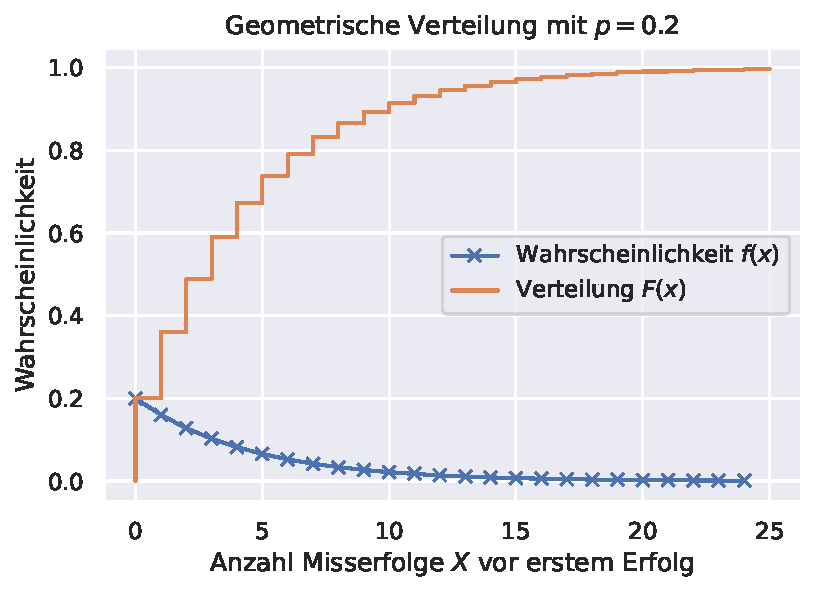
\includegraphics[width=0.5\textwidth]{data/geometric-distr.pdf}%
        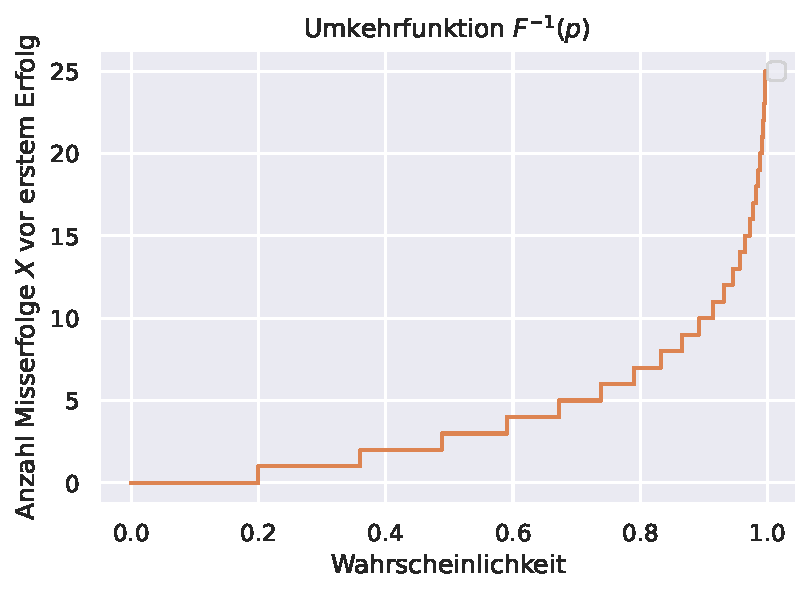
\includegraphics[width=0.5\textwidth]{data/geometric-distr-inv.pdf}
    \end{center}

    \caption{
        Wahrscheinlichsverteilung und kumulative Verteilungsfunktion einer geometrischen Verteilung mit Parameter $p = 0.2$ (links).
        Die rechte Abbildung zeigt die \glqq Umkehrfunktion\grqq{} $F^{-1}(p)$ der kumulativen Verteilungsfunktion $F(x)$.
    }
    \label{fig:geometric-distr}
\end{figure}

Die Inversionsmethode (inversion transform method) ist ein allgemeines Verfahren, um eine uniforme Zufallsvariable in eine andere Verteilung zu übersetzen.
Wir betrachten die Methode hier am Beispiel der geometrischen Verteilung.
In \cref{fig:geometric-distr} ist die Wahrscheinlichkeitsverteilung $f(\ell)$ und die kumulative Verteilungsfunktion $F(\ell)$ einer geometrischen Verteilung mit Parameter $p = 0.2$ gezeigt.
%
%Da $f(\ell)$ ist eine Wahrscheinlichkeitsverteilung ist, muss $\sum_{\ell=0}^{\infty} f(\ell) = 1$ gelten.
Betrachten wir die konkreten ersten drei Werte der Funktionen:

\begin{center}
    \begin{tabular}{l|p{0.2\textwidth}p{0.25\textwidth}p{0.35\textwidth}}
                  & $\ell = 1$ & $\ell = 2$              & $\ell = 3$                              \\\hline\hline
        $f(\ell)$ & $p =0.2$   & $(1 {-} p)p = 0.16$     & $(1 {-} p)^2p = 0.128$                  \\
        $F(\ell)$ & $p =0.2$   & $p{+}(1 {-} p)p = 0.36$ & $p{+}(1 {-} p)p{+}(1 {-} p)^2p = 0.488$
    \end{tabular}
\end{center}
\vspace{1em}


Ein Generator sollte also z.B. den Wert $0$ mit Wahrscheinlichkeit 20\,\% ausgeben.
Da wir einen determistischen Algorithmus konstruieren möchten, brauchen wir eine Quelle für den Zufall:
wir erwarten eine uniforme Zufallsvariable $U \in [0, 1]$ als Eingabe.
Wir können also z.B. prüfen:
\begin{itemize}
    \item Wenn $U < 0.2$ ist und dann den Wert $0$ zurückgeben.
          Da $U$ uniform verteilt ist, ist die Wahrscheinlichkeit für $U < 0.2$ genau $0.2$.

    \item Falls nicht prüfen wir, ob $U < 0.36 = f(0) + f(1) = F(1)$ ist. Falls ja, geben wir den Wert $1$ zurück.
          Da $U$ uniform verteilt ist, wir aber wissen, dass $U$ nicht kleiner als $0.2$ ist, ist die Wahrscheinlichkeit $\prob{U < 0.36 | U > 0.2} = 0.16 = f(1)$.

    \item Diesen Prozess setzen wir fort, bis wir das passende Intervall gefunden haben.
\end{itemize}

Die graphische Interpretation ist also die folgende:
In \cref{fig:geometric-distr} (rechts) ist die Umkehrfunktion~$F^{-1}(p)$ der kumulativen Verteilungsfunktion $F(x)$ gezeigt.
Wir werfen nun mittels der zufälligen Eingabe $U$ einen Punkt auf der $x$-Achse und schauen, welchen Wert $F^{-1}(U)$ hat --- dies ist unsere Ausgabe.

Im folgenden Theorem wird die Inversionsmethode formalisiert, wobei wir vereinfachend einige Annahmen treffen.
Die Methode lässt sich aber auch auf andere $\Omega$ (inklusive kontinuierliche) und nicht streng monotone $F(x)$ verallgemeinern.

\begin{theorem}
    Sei $X \in \Omega$ eine diskrete Zufallsvariable und $f(x)$ und $F(x)$ ihre Wahrscheinlichkeitsverteilung sowie die kumulative Verteilungsfunktion.
    Vereinfachend sei $\Omega$ total geordnet und $F(x)$ streng monoton steigend.
    Dann existiert die Umkehrfunktion $F^{-1}(x)$ mit $F^{-1}(F(x)) = x$.
    Sei $U$ eine uniforme Zufallsvariable aus $[0, 1]$.
    Dann ist $X' = F^{-1}(U)$ eine Zufallsvariable mit der Wahrscheinlichkeitsverteilung $f(x)$.
\end{theorem}

\begin{proof}
    \noindent Da $F$ streng monoton ist, existiert die Umkehrfunktion $F^{-1}$ und es gilt:
    \begin{equation}\label{eq:inverse-apply-inverse}
        F(x) = p
        \quad\Leftrightarrow\quad F^{-1}(F(x)) = F^{-1}(p)
        \quad\Leftrightarrow\quad x = F^{-1}(p)
    \end{equation}

    \noindent Daraus folgt dann direkt:
    \begin{eqnarray}
        \prob{X' \le x} &\stackrel{\text{Inv. Method}} = & \prob{F^{-1}(U) \le x} \\
        &\stackrel{(\ref{eq:inverse-apply-inverse})}{=}& \prob{U \le F(x)} \\
        &\stackrel{\prob{U < z} = z \forall z \in [0, 1]}=& F(x) \\
        &\stackrel{\text{Def.} F(X)}=& \prob{X \le x} \hspace{5em}\hfill \qedhere
    \end{eqnarray}
\end{proof}

\bigskip
\bigskip

Zurück \aside{Inversionsmethode für geometrische Verteilung} zur geometrischen Verteilung mit $f(\ell) = (1-p)^\ell p$.
ObdA sei $0 < p < 1$ (da $X$ sonst eine Konstante ist).
Die kumulative Verteilungsfunktion lautet
\begin{equation}
    F(\ell)
    \ =\ p \sum_{i=0}^\ell (1-p)^\ell
    \ \stackrel{(*)}{=} \ p \frac{1 - (1-p)^{\ell+1}}{\underbrace{1 - (1-p)}_{=p}}
    \ = \ 1 - (1-p)^{\ell+1},
\end{equation}
wobei wir in $(*)$ die geschlossene Form der $\ell$-ten Partialsumme der geometrischen Reihe nutzen $\sum_{i=0}^\ell x^\ell = (1 - x^{\ell+1})/(1 - x)$.
Nun berechnen die Umkehrfunktion $F^{-1}(U) = \ell$ indem wir $F(\ell) = U$ setzen und nach $U$ umformen:
\begin{eqnarray}
    U &=& F(\ell) = 1 - (1-p)^{\ell+1} \\
    \Leftrightarrow (1-p)^{\ell+1} &=& 1 - U \\
    \Leftrightarrow  (\ell+1) \log(1-p)  &=& \log(1 - U) \\
    \Leftrightarrow  F^{-1}(U) := \log_{1-p}(1 - U) - 1 &=& \ell
\end{eqnarray}

\noindent
\textcolor{red}{TODO: Hier fehlt Runden!}
Zusammenfassen erzeugt \cref{alg:sample-geometric} eine geometrische Zufallsvariable $X$ mit Parameter $p$ in Zeit $\Oh{1}$:

\begin{algorithm}[H]
    \If{p=0}{Gebe $\infty$ zurück}
    \ElseIf{p=1}{Gebe $0$ zurück}
    \Else{$U \gets \text{ziehen uniform aus $[0, 1)$}$\;
    Gebe $\log_{1-p}(1 - U) - 1$ zurück.}
    \caption{Ziehen einer geometrischen Zufallsvariable}
    \label{alg:sample-geometric}
\end{algorithm}

\section{Effizientes Ziehen von \Gnm Graphen}
Trotz der strukturellen Ähnlichkeiten zwischen \Gnp und \Gnm Graphen unterscheiden sich ihre Generatoren signifikant.
Grund hierfür ist, dass während \Gnp \emph{in Erwartung} $n^2p$ Kanten erzeugen, müssen wir für \Gnm Generatoren sicherstellen, dass exakt $m$ zufällige Kanten produziert werden.

Ähnlich wie zuvor, reduzieren wir das Ziehen der richtigen Position von \emph{Einsen} in der Adjazenzmatrix auf den eindimensionalen Fall.
Im Folgenden werden wir also folgendes äquivalentes Problem lösen:
Ziehe uniform ohne Zurücklegen $k$ Elemente aus einer Menge $S = \set{s_1, \ldots, s_n}$ mit $|S| = n > k$.

\clearpage

\subsection{Reservoir Sampling}
Reservoir Sampling ist eine allgemeine Technik, die es uns erlaubt $k$ Elemente aus einem Datenstrom zu ziehen.
Hierbei müssen wir anfangs \emph{nicht} wissen, wie viele Elemente insgesamt im Strom sind.\footnote{
    Ein praktischer Anwendungsfall sind z.B. Iteratoren oder Generatoren, die in vielen Programmiersprachen genutzt werden.
    In Rust ist z.B. \texttt{rand::IteratorRandom::choose\_multiple} mittels Reservoir Sampling implementiert.
}
Im konkreten Fall besteht der Datenstrom also aus allen $s_i$ in beliebiger Reihenfolge.
Vereinfachend können wir also annehmen, dass der Strom mindestens $k$ Elemente enthält.

\begin{algorithm}[H]
    \KwIn{Eingabe: Datenstrom~$S$, Stichprobengröße: $k$}
    \KwOut{Array $R[1..k]$ mit $k$ zufällig ausgewählten Elementen}

    Initialisiere ein anfangs leeres Array $R$ mit Kapazität $k$\;

    \While{$|R| < k$}{
        $x \gets \text{nächstes Element aus $S$}$\;
        Füge $x$ an $R$ an\;
    }

    Setze $i = k$\;
    \While{$S$ nicht leer}{
        $x \gets \text{nächstes Element aus $S$}$\;
        $i \gets i + 1$\;
        $j \gets \text{ziehe uniform aus $[1, i]$}$\;
        \If{$j \le k$}{
            Ersetze $R[j] \gets x$\;
        }
    }

    Gebe $R$ zurück

    \caption{Reservoir Sampling}
    \label{algo:reservoir-sampling}
\end{algorithm}

\bigskip
\bigskip

\noindent
In \cref{thm:reservoir-sampling} zeigen wir die Korrektheit von \cref{algo:reservoir-sampling} für nur $k = 1$:
\begin{theorem}\label{thm:reservoir-sampling}
    \Cref{algo:reservoir-sampling} liefert für $k=1$ ein uniform gewähltes Element aus $S$.
\end{theorem}
\begin{proof}
    Sei $n$ die Länge des Stroms und seien $s_1, \ldots, s_n$ die Elemente in der Reihenfolge wie sie aus dem Strom gelesen werden; oBdA gelte $s_i = s_j \ \Leftrightarrow\ i = j$.
    Sei $R$ die Zufallsvariable, die die Ausgabe des Algorithmus modelliert.
    Dann ist zu zeigen, dass $\prob{R = s_i} = 1 / n$ für alle $1 \le i \le n$.
    \begin{eqnarray}
        \prob{R = s_i} &=& \prob{\text{$s_i$ wird in Runde~$i$ gewält}} \cdot \prob{\text{$s_i$ wird nicht ersetzt}} \\
        &=& \frac{1}{i} \cdot \underbrace{\prod_{j=i+1}^n \frac{j-1}{j}}_{\text{Teleskopprodukt}}
        = \frac{1}{i} \cdot \frac{i}{n} = \frac{1}{n}
    \end{eqnarray}

    \noindent Insbesondere gilt also, dass $\prob{R = s_i} = 1/n$ unabhängig von $i$ oder $s_i$ ist.
\end{proof}

\begin{exercise}
    Zeige die Korrektheit von \cref{algo:reservoir-sampling} indem du den Beweis von \cref{thm:reservoir-sampling} auf $k \ge 1$ verallgemeinerst.
\end{exercise}

Wir können also \Gnm Graphen mittels Reservoir Sampling erzeugen.
Allerdings müssen wir pro potentieller Kante konstant viel Arbeit verrichten.
Somit folgt eine Laufzeit von $\Theta(n^2)$.

\subsection{Ziehen mit Sprüngen}

\subsection{Ziehen mit Hashsets}


\section{Kritische Punkte}


\section{Gradverteilung}
